\chapter{Техническое задание}

Спроектировать и провести моделирование двухканальной приёмной ячейки с управляемым фазовым сдвигом в каналах и фильтрацией в соседних каналах.
Структурная схема проектируемого устройства представлена на Рис.~\ref{fig:tor_structure_schematic}.

\begin{figure}[!ht]
	\centering
	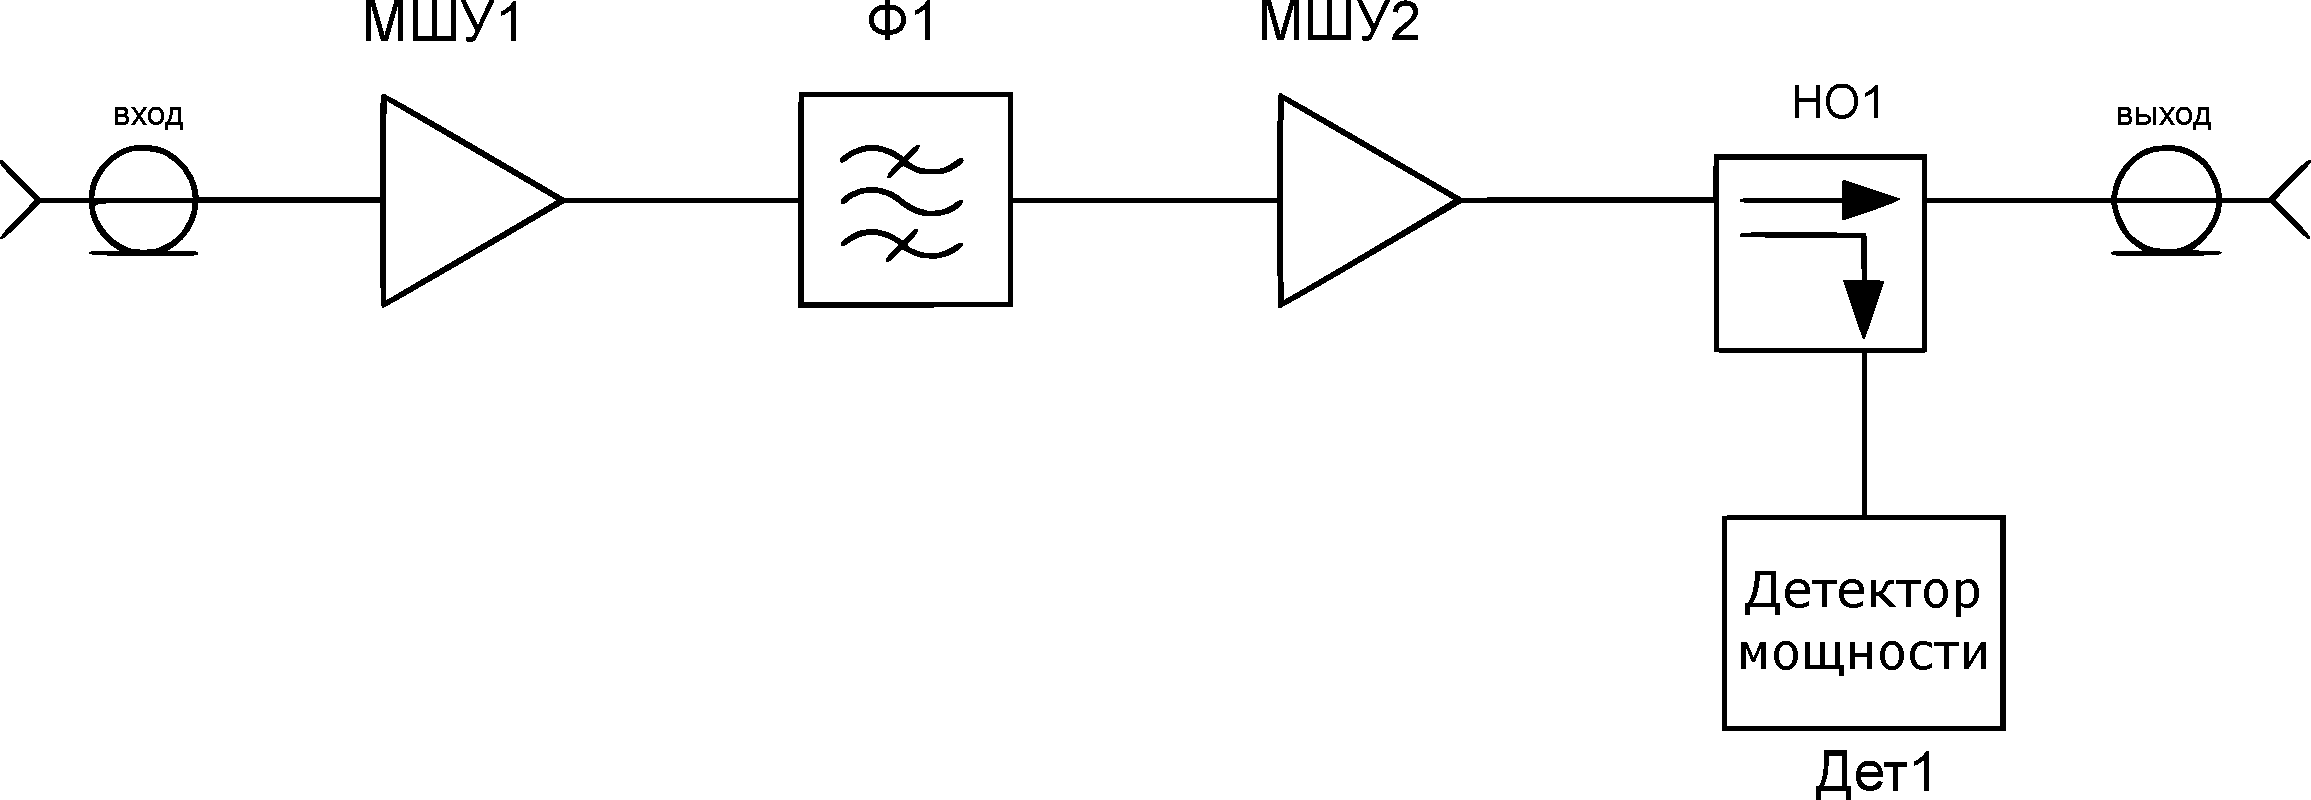
\includegraphics[width=\textwidth]{MainStrSch.pdf}
	\caption{Структурная схема проектируемого устройства}%
	\label{fig:tor_structure_schematic}
\end{figure}

\textit{Общие условия и пояснения:}
\begin{enumerate}
	\item
	КСВН по всем ВЧ-входам и ВЧ-выходам должен быть не более $1.5$ в рабочей полосе частот.
	\item
	Усилители МШУ1 и МШУ2 не обязательно должны быть одним устройством, могут являться каскадными.
	\item
	Предпочтительно чтобы первым устройством был фильтр Ф1, однако, если из-за потерь на фильтре Ф1 невозможно удовлетворить на Кш, то первый МШУ с минимальным коэффициентом шума можно поставить первым.
	\item
	Рабочий диапазон частот $F_{p1} \ldots F_{p2}$ определяется как размах $\Delta F_\text{-3~dB}$ относительно центральной частоты $F_c$, т.е. $F_{p1} = F_c - 0.5 \Delta F_\text{-3~dB}$ и $F_{p2} = F_c + 0.5 \Delta F_\text{-3~dB}$.
	\item
	Ячейка должна быть способна корректно измерять возможные значения входной мощности Pin. Это означает, что данный диапазон возможной входной мощности с учетом прохождения через канал (МШУ, ППФ, ответвление в вторичное плечо НО) должен попадать в динамический диапазон измеряемой мощности детектора мощности в рабочей полосе частот
\end{enumerate}

\begin{figure}[!ht]
	\centering
	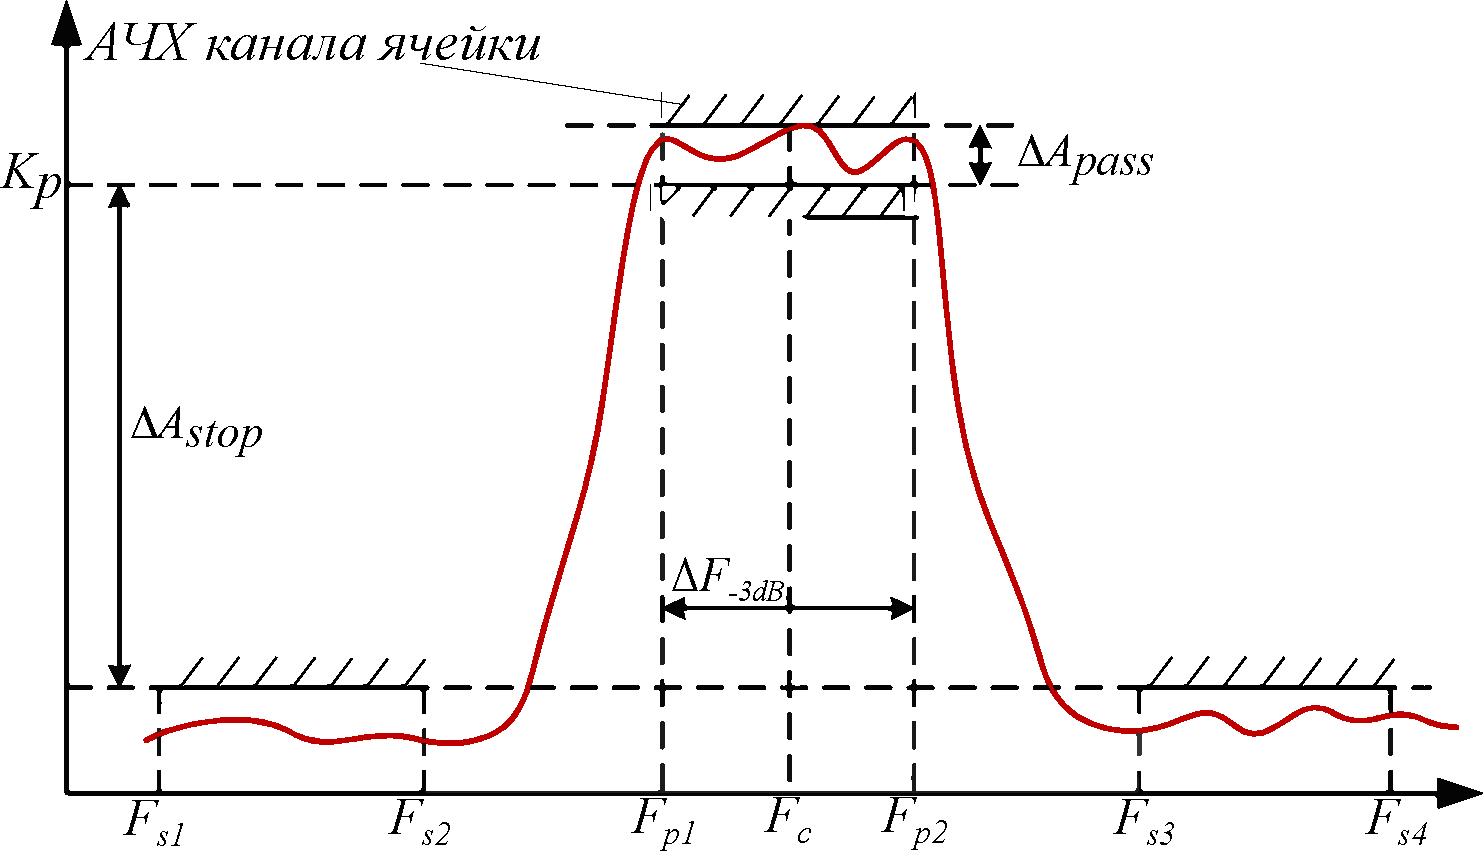
\includegraphics[width=\textwidth]{TZ.pdf}
	\caption{Пояснение к ТЗ на АЧХ канала}%
	\label{fig:tor_response}
\end{figure}



\begin{table}[!h]
	%\captionsetup{singlelinecheck=off, justification=raggedright}
	\begin{center}		
		\caption[Вариант задания]{Вариант задания}\label{tab:tasktab}
		\begin{tabularx}{0.95\textwidth}{ !{\vrule width 2pt}*{4}{>{\centering\arraybackslash}X|}>{\centering\arraybackslash}X!{\vrule width 2pt}}
			\bhline{2}
			Fc, ГГц & 
			Kp, дБ, не менее & 
			$\Delta F_\text{-3~dB}$ГГц, не  менее & 
			\multicolumn{2}{|c!{\vrule width 2pt}}{$\Delta A_\text{pass}$, дБ, не более} \\ \hline
			%
			8.5&39&0.5&\multicolumn{2}{|c!{\vrule width 2pt}}{3}\\ \bhline{2}
			%
			Нижний диапазон запирания, $F_{S1} \ldots F_{S2} \text{, ГГц}$ &
			Верхний диапазон запирания, $F_{S3} \ldots F_{S4} \text{, ГГц}$ &
			$\Delta A_\text{stop} \text{, дБ}$, не менее &Кш, дБ, не более & Диапазон ожидаемых входных мощностей, Pin, дБмВт\\ \hline
			%
			$7.35\ldots7.85$&$9.1\ldots9.6$&33&3.3&$-42\ldots-15$\\ \bhline{2}
		\end{tabularx}
	\end{center}
\end{table}

Проектировать будем на подложке RO4003 0.5 oz ED 20 mil (Er = 3.38, Ur = 1, Tand = 
0.0027, T = 17 мкм, H = 0.508 мм).